\begin{abstract}
Meta-SAEs' decomposition of a parent sparse autoencoder's (SAE) decoder directions into meta-latents has been used to show that SAE latents are not always atomic.
To our knowledge, no published study asks whether meta-SAEs are reproducible across seeds.
We train meta-SAEs on a GPT-2 small reference setup adapted from \citet{leask2025canonical} and, at widths 1/4 to 1/128, on a model size sweep of five Gemma Scope 2 parents (trained on Gemma 3 270M to 27B).
We also train ``noise twin'' meta-SAEs on unit-normalized draws of a Gaussian fitted (mean and covariance) to the real parent's unit decoder directions, then use this baseline to compute excess agreement as real raw agreement---where agreement is the mean decoder cosine of one-to-one matched meta-latents over all pairs of eight seeds---minus the noise twins'.
In the reference, 64.0\% of meta-latents recur at cosine 0.7 or more, against 0.07\% for the noise twins.
On the Gemma 3 size sweep, at most 29.9\% recur while a bifurcated trend in width appears: by excess agreement, width 1/4 is best for sizes 270M and 1B (at most 7.7\% recurring) while widths 1/32 to 1/128 all beat 1/4 for sizes 4B to 27B (with 1.8 to 3.3 times the recurring fraction at width 1/4).
This contrasts with how raw agreement peaks at width 1/128 for four of five sizes, pointing to excess agreement as a promising metric for choosing meta-SAE settings.
\end{abstract}

\section{Introduction}

A sparse autoencoder (SAE) trained to reproduce the decoder directions of a parent SAE with fewer latents (meta-latents) is called a meta-SAE, which was introduced by \citet{bussmann2024metasae}. Meta-latents can be interpreted as representing more general concepts related to the latent's concept. For example, an ``Einstein'' latent might deconstruct into meta-latents like ``scientist'', ``prominent figures'', and ``Germany''. This idea was used by \citet{leask2025canonical} to argue that larger SAEs' latents are not always atomic, while SAE stitching showed that smaller SAEs' latents are incomplete in representing all features of the LLM. The underlying mechanism of meta-SAEs has been used to score the atomicity of SAEs \citep{korznikov2025ortsae}, to train atomicity-conscious SAEs \citep{levinson2026metasaes}, and to create cascaded SAEs for jointly learning a two-level dictionary \citep{zhao2026saepp}. However, all these studies assume reproducibility across meta-SAE seeds.

\citet{paulo2025sae} found partial seed reproducibility for ordinary SAEs, but no known studies to date investigate similarly for meta-SAEs. Studies have also typically not swept meta-SAE width and instead used conventional choices such as 1/4 \citep{bussmann2025matryoshka,korznikov2025ortsae} or 1/2 \citep{zhao2026saepp}. Thus, it matters whether the configuration adapted from \citet{leask2025canonical}---our reference---is reproducible across seeds to begin with and how seed-reproducible meta-SAEs are for various widths and underlying LLM sizes.

\begin{figure}[t]
  \centering
  \begin{tikzpicture}[
  font=\footnotesize,
  >={Stealth[length=3.4pt,width=3pt]},
  box/.style={draw, rounded corners=1.5pt, line width=0.5pt, align=center, inner xsep=3.5pt, inner ysep=2pt, minimum height=0.64in},
  real/.style={box, draw=acc!85!black, fill=acc!10},
  twin/.style={box, draw=black!80, fill=white},
  stack/.style={draw, rounded corners=1.5pt, line width=0.5pt, fill=white},
  flow/.style={->, line width=0.5pt},
  lane/.style={anchor=south west, inner sep=0pt, yshift=2.5pt, font=\footnotesize\bfseries},
]
\definecolor{acc}{RGB}{26,95,160}
\def\dy{1.0in}
\def\g{0.125in}
% real lane
\node[real, minimum width=0.56in] (r1) {Parent\\decoder\\rows\\$n\times d$};
\node[real, minimum width=0.50in, right=\g of r1] (r2) {Unit\\rows};
\node[real, minimum width=0.58in, right=\g of r2] (r3) {Train, val,\\test rows\\80/10/10};
\node[real, minimum width=0.84in, right=\g of r3] (r4) {Meta-SAE\\BatchTopK, $k{=}4$\\$wn$ meta-latents\\on train rows};
\node[real, minimum width=0.70in, right=\g of r4] (r5) {One-to-one\\matching\\28 seed pairs};
\node[real, minimum width=0.60in, right=\g of r5] (r6) {Real\\agreement};
% twin lane
\node[twin, minimum width=0.56in, below=\dy of r1.center, anchor=center] (t1) {Gaussian\\rows\\$n\times d$};
\node[twin, minimum width=0.50in, right=\g of t1] (t2) {Unit\\rows};
\node[twin, minimum width=0.58in, right=\g of t2] (t3) {Train\\rows\\80\%};
\node[twin, minimum width=0.84in, right=\g of t3] (t4) {Meta-SAE\\BatchTopK, $k{=}4$\\$wn$ meta-latents\\on train rows};
\node[twin, minimum width=0.70in, right=\g of t4] (t5) {One-to-one\\matching\\28 seed pairs};
\node[twin, minimum width=0.60in, right=\g of t5] (t6) {Twin\\agreement};
\begin{pgfonlayer}{background}
  % seeds as a stack of cards behind each meta-SAE box
  \foreach \n/\c in {r4/acc!85!black,t4/black!80} {
    \foreach \s in {3,6} {
      \draw[stack, draw=\c] ($(\n.north west)+(\s*0.7pt,\s pt)$) rectangle ($(\n.north east)+(-\s*0.7pt,\s pt-8pt)$);
    }
  }
\end{pgfonlayer}
\node[anchor=south, inner sep=1pt] at ([yshift=8pt]r4.north) {8 seeds};
\node[anchor=south, inner sep=1pt] at ([yshift=8pt]t4.north) {8 seeds};
\foreach \a/\b in {r1/r2,r2/r3,r3/r4,r4/r5,r5/r6,t1/t2,t2/t3,t3/t4,t4/t5,t5/t6}
  \draw[flow] (\a.east) -- (\b.west);
% twin rows take their mean and covariance from the parent's unit rows
\coordinate (mid) at ($(r2.south)!0.5!(t1.north)$);
\coordinate (cm) at (r2.south |- mid);
\coordinate (land) at ([xshift=-0.1in]t1.north east);
\draw[flow, dashed] (r2.south) -- (cm) -- (land |- mid) -- (land);
\node[anchor=west, inner sep=1pt] at ([xshift=3pt]cm) {mean, covariance};
% columns 1 to 3 of both lanes are shared by all widths and seeds
\coordinate (bl) at ([yshift=-6pt]t1.south west);
\coordinate (br) at ([yshift=-6pt]t3.south east);
\draw[line width=0.5pt, black!80] (bl |- t1.south) -- (bl) -- (br) -- (br |- t3.south);
\node[below, inner sep=1.5pt, text=black!80] at ($(bl)!0.5!(br)$) {shared by all widths and seeds};
% excess
\node[draw=acc!85!black, fill=acc, text=white, rounded corners=1.5pt, line width=0.5pt, align=center, inner xsep=3.5pt, inner ysep=2pt,
      minimum width=0.62in, minimum height=1.64in, anchor=west]
  (ex) at ($(r6.east)!0.5!(t6.east)+(\g,0)$) {Excess\\agreement\\[3pt]real${}-{}$twin};
\draw[flow] (r6.east) -- (r6.east -| ex.west);
\draw[flow] (t6.east) -- (t6.east -| ex.west);
\node[lane] at (r1.north west) {Real};
\node[lane] at (t1.north west) {Twin};
\end{tikzpicture}

  \caption{The excess agreement measurement pipeline for one parent SAE and meta-SAE width. The parent's $n$ decoder rows (dimension $d$) are scaled to unit length and, for a Gemma Scope 2 parent, split into training, validation, and test rows. Meta-SAEs with $wn$ meta-latents ($w$ is the width, as 1/4 to 1/128 for the main widths) train on the training rows with eight seeds that differ only in initial weights and shuffle order. Twin runs (lower lane) train on Gaussian rows but are validated and tested on the real rows.}
  \label{fig:pipeline}
\end{figure}

We run eight seeds for each meta-SAE configuration (width and LLM size) and then measure the agreement amongst them, where agreement is the mean cosine of Hungarian-matched pairs of decoder directions between pairs of unique seeds (Figure~\ref{fig:pipeline}). The seed-reproducibility of the reference configuration uses their parent SAE of GPT-2 small and meta-SAE settings adapted from theirs. The width-and-size sweep is done with five Gemma Scope 2 parent SAEs \citep{mcdougall2025gemmascope2} of the middle layers of respective Gemma 3 model sizes \citep[270M, 1B, 4B, 12B, and 27B;][]{gemmateam2025gemma3,googledeepmind2025gemma3card}, across six widths (1/4 to 1/128). To distinguish agreement from Hungarian-matched noise, we train noise twin meta-SAEs with the same settings as each meta-SAE configuration by training on unit-length Gaussian draws of the parent SAE's unit-length decoder directions and then record excess agreement (setup agreement minus noise twin agreement).

To our knowledge, this is the first width sweep of meta-SAE seeds' excess agreement. Our findings and contributions are as follows:
\begin{itemize}
  \item \textbf{Reference.} The reference configuration averages 64.0\% of meta-latents shared per seed pair (using one-to-one matching with at least 0.7 decoder cosine, which we call the recurring fraction) against 0.07\% for the noise twins. For the width-size sweep---whose parent SAEs are a different type, number of latents per hidden dimension, and underlying LLM, among other settings---the recurring fraction is less than a third.
  \item \textbf{Width by size.} For Gemma 3 270M and 1B, meta-SAE width 1/4 yields the highest excess agreement---although under 8\% of meta-latents recur---while smaller widths show a trend of lower, even non-positive, excess agreements. For 4B to 27B, widths 1/32 to 1/128 yield higher excess agreements than that of 1/4. Each main sweep width at every Gemma 3 model size has a meaningfully higher recurring fraction than its noise twins.
  \item \textbf{Noise twins.} While width 1/128 dominates raw agreement for four of the five Gemma 3 sizes, noise twin agreement over width is generally U-shaped for each model size. This heavily impacts which width has the best excess agreement when moving from 270M to 12B.
  \item \textbf{Controls.} Given equal training steps, comparisons between meta-SAEs trained on three randomly drawn quarters of the 4B parent's rows and on the released 16,384-latent Gemma Scope 2 SAE (same 4B layer) indicate that none of width, meta-latent count or row count alone determines excess agreement.
  \item \textbf{In-practice consequences.} When using meta-SAEs on different parent SAEs, one should consider excess agreement over noise twins instead of raw agreement and consider narrower widths (at least on Gemma Scope 2) for larger LLMs.
\end{itemize}

\section{Related work}

\begin{table}[t]
  \caption{Published meta-SAE setups. Width is the meta-latent count as a percentage of the parent SAE's latent count. \citet{leask2025canonical} and \citet{bussmann2024metasae} use the same parent SAE and meta-latent count. ``Frozen parent'' means the meta-SAE is trained on a finished parent SAE while ``joint'' means the two are jointly trained. \citet{maiwald2025decodeglm} give no width percentage because they train on an unstated number of positive-F1 parent latents.}
  \label{tab:published}
  \centering\small
  \begin{tabular}{@{}llll@{}}
    \toprule
    Work & Parent SAE (latents) & Meta-latents (width) & Training \\
    \midrule
    \citet{bussmann2024metasae} & GPT-2 small, layer 8 (49,152) & 2,304 (4.7\%) & frozen parent \\
    \citet{bussmann2025matryoshka} & SAEs (2,304 to 36,864) & 576 to 9,216 (25\%) & frozen parent \\
    \citet{korznikov2025ortsae} & Gemma 2 2B, Llama 3 8B (65,536) & 16,384 (25\%) & frozen parent \\
    \citet{levinson2026metasaes} & GPT-2 large, layer 20 (20,480) & 1,800 (8.8\%) & joint \\
    \citet{zhao2026saepp} & 3 multimodal models (20,000) & 10,000 (50\%) & joint \\
    \citet{maiwald2025decodeglm} & Nucleotide Transformer 500M (unstated) & 128 & frozen parent \\
    \bottomrule
  \end{tabular}
\end{table}

\paragraph{Meta-SAEs and their widths.}
Meta-SAE width has been swept before, by \citeauthor{maiwald2025decodeglm} (\citeyear{maiwald2025decodeglm}; Table~\ref{tab:published}), but by balancing L0 sparsity against explained variance instead of agreement between seeds. \citet{levinson2026metasaes} left the investigation of meta-SAE width's effect on dictionary compression to future work, but no known studies explicitly research meta-SAE seed reproducibility.

\paragraph{Agreement between SAE seeds.}
\citet{paulo2025sae} is this paper's closest prior study, in which they treated latents as shared if one-to-one matching for encoder and decoder rows both agree and achieve a cosine of 0.7 or more, and then found shared fractions of about 0.8 (32 latents) and 0.3 (131K latents) for Pythia 160M, and 0.3 (131K latents) for Llama 3 8B. \citet{gerasimov2026unstable} observed only partial seed reproducibility for SAEs and that whether larger latent counts lowered or raised reproducibility depended on the model and layer. Their study varied SAE latent count and model layer for its effect on the fraction of features whose best match (many to one, cosine 0.7 or more) reappears in 95\% or more other seeds, while using an SAE trained on an untrained GPT-2 as a null baseline. Studies like \citet{song2026consistency} and \citet{cho2025faithfulsae} jointly vary other settings besides model size, such as choice of model layer and TopK's K. \citet{song2026consistency} also tuned TopK's K and penalty for PW-MCC. \citet{choi2026beyond}, however, vary latent count on four models while using model layers with the same hidden size and saw seed agreement mostly fall for larger SAE latent counts. When measuring seed agreement against a random-unit-vector baseline computed by formula, \citet{liu2026timescale} found that longer training, on Pythia 410M layer 21, narrowed seed agreement gaps between different widths while agreement kept rising without a plateau. Our agreement measure is taken from \citeauthor{fel2025archetypal}'s \citeyearpar{fel2025archetypal} one-to-one matched mean cosine, but without sign flips.

\paragraph{Choosing size by stability.}
For older, classical methods such as NMF, the number of components was chosen by how stable sample clusters and dictionaries are across restarts \citep{brunet2004metagenes,wu2016stanmf}, and \citet{greene2014howmany} chose topic count in topic models by one-to-one matched agreement over document subsamples. \citeauthor{horn1965rationale}'s \citeyearpar{horn1965rationale} parallel analysis is a precedent of subtracting a sampling error, estimated given random data, from eigenvalues to pick the number of factors in factor analysis. Similar to \citet{gerasimov2026unstable}, we train noise twins; they have as many decoder rows as the real data too, similar to \citeauthor{horn1965rationale}'s uncorrelated normal data \citep{dinno2009exploring}. But unlike \citet{gerasimov2026unstable} and \citet{liu2026timescale}, the noise twin's training rows are normalized Gaussian draws with the same mean and covariance as the parent's normalized decoder rows.

\section{Setup}

\paragraph{Meta-SAEs.}
As in \citet{leask2025canonical}, we use BatchTopK \citep{bussmann2024batchtopk} meta-SAEs and keep the $kB$ largest activations in each batch of $B$ rows ($k$ = 4 on average).
The training rows are scaled to unit length.
For the reproducibility of the reference configuration, \citeauthor{leask2024metasaerelease}'s \citeyearpar{leask2024metasaerelease} released meta-SAE obtains an explained variance of 0.5514 in our code while our eight seeds' meta-SAEs (Appendix~A) report 0.5504 to 0.5511.

\paragraph{Parent SAEs.}
The five main parent SAEs are 65,536-latent Gemma Scope 2 \texttt{l0\_medium} SAEs (JumpReLU, \citealp{rajamanoharan2024jumprelu}; \citealp{mcdougall2025gemmascope2}; released configs: L0 60) for pretrained Gemma 3 \citep{gemmateam2025gemma3,googledeepmind2025gemma3card} on the residual stream after block $N/2$ of $N$ (Table~\ref{tab:parents}).
\citet{lmit2025gemmascope2blog} report Matryoshka training for the release but not which SAEs or widths use it.
Since all five parent SAEs have the same latent count, widths 1/4 to 1/128 correspond to 16,384 to 512 meta-latents for each parent.
Two 16k-latent parents, at 4B and 270M, serve as controls (Section~4.3).

\begin{table}[t]
  \caption{The five main parent SAEs and two 16k control parents, reported with their layers counted from 0 \citep{mcdougall2025gemmascope2} of $N$ blocks \citep{googledeepmind2026gemmalib}, alongside tokens and image input \citep{gemmateam2025gemma3,googledeepmind2025gemma3card}.}
  \label{tab:parents}
  \centering
  \small
  \begin{tabular}{@{}lrrrrrc@{}}
    \toprule
    Gemma 3 parent & Latents & Hidden size & Layer & Latents per hidden dim. & Tokens & Image input \\
    \midrule
    270M & 65,536 & 640 & 9 of 18 & 102.4 & 6T & no \\
    1B & 65,536 & 1,152 & 13 of 26 & 56.9 & 2T & no \\
    4B & 65,536 & 2,560 & 17 of 34 & 25.6 & 4T & yes \\
    12B & 65,536 & 3,840 & 24 of 48 & 17.1 & 12T & yes \\
    27B & 65,536 & 5,376 & 31 of 62 & 12.2 & 14T & yes \\
    4B 16k & 16,384 & 2,560 & 17 of 34 & 6.4 & 4T & yes \\
    270M 16k & 16,384 & 640 & 9 of 18 & 25.6 & 6T & no \\
    \bottomrule
  \end{tabular}
\end{table}

\paragraph{Training.}
Each Gemma Scope 2 parent has its unit rows partitioned into one 80/10/10 split that is reused for every width and seed.
We use Adam \citep{kingma2015adam} with a learning rate of 3e-3 for every Gemma Scope 2 run (except the 1e-3 rate check in Section~4.4), alongside betas 0.9 and 0.999, batches of 4,096, and gradient clipping at norm 1, while the meta-SAE decoder rows are rescaled to unit length.
The learning rate was decided after tuning (Appendix~B).
To recover dead latents, AuxK \citep{gao2025scaling}, at weight 1/32, trains meta-latents that have been inactive for 5 epochs.
Each sweep run (not the controls or the rate check) trains for 2,000 epochs, and then trains for another 2,000 epochs if our length rule (Appendix~C) finds that validation MSE still falls or real agreement still rises meaningfully.

\paragraph{Noise twins.}
Each parent's noise twin is one set of Gaussian rows, as many as the parent's rows, drawn with the mean and covariance of the parent's unit rows and rescaled to unit length.
For a Gemma Scope 2 parent, twin meta-SAEs of every width and seed train on an 80\% split of these rows, as many as the real training rows, while the reference twin trains on all of them.
Note that the sampling, 80\% training subset, and rescaling shift the noise twin's statistics, in that the largest covariance eigenvalue of its training rows is 6.0\% to 9.5\% below that of each parent's unit rows for the five main parents (18.4\% for the 4B 16k and 9.4\% for the 270M 16k).

\paragraph{Measuring agreement.}
Decoder rows between two meta-SAE runs are matched one-to-one to maximize signed cosine \citep{kuhn1955hungarian}, similar to \citet{fel2025archetypal}.
Raw agreement is then computed as the matched cosine averaged over meta-latents and then over the 28 seed pairs.
Excess agreement is raw agreement with noise twin raw agreement subtracted:
\begin{equation}
  A = \operatorname{mean}_{i<j} \max\nolimits_{\pi} \operatorname{mean}_{l} \cos(u_{i,l}, u_{j,\pi(l)}), \qquad \Delta A = A_{\mathrm{real}} - A_{\mathrm{twin}},
  \label{eq:agreement}
\end{equation}
where $u_{i,l}$ is decoder row $l$ for seed $i$ and $\pi$ a bijective permutation mapping of the decoder row indices.
The average share (over the seed pairs) of matched pairs at cosine 0.7 or more is named the recurring fraction.
Using \citeauthor{bussmann2024batchtopk}'s \citeyearpar{bussmann2024batchtopk} activation threshold fitted after training, we measure live-only agreement by only matching meta-latents that activate for at least one training row.
Uncertainty is reported as 90\% leave-one-seed-out jackknife t intervals with 7 degrees of freedom \citep{efron1979bootstrap}, which measure seed-to-seed variation for a fixed parent and split, with the Gaussian rows also held fixed.
We also use them to define near-best widths: the top width, which has the largest excess agreement, and any width whose 90\% interval on its gap to the top width contains 0.
The seeds cannot show that such a width is worse than the top.
At each model size, the six main widths are compared twice, once at 2,000 epochs and once at each width's longest length.
Both comparisons are repeated at 4B with width 1/256 added.

\paragraph{Experiments.}
The reference configuration reproducibility experiment trains meta-SAE seeds of width 3/64 (2,304 meta-latents) on all 49,152 unit rows of \citeauthor{bloom2024gpt2featuresplitting}'s \citeyearpar{bloom2024gpt2featuresplitting} GPT-2 small SAE's block 8 input \citep{radford2019language}, which has 768 hidden dimensions.
\citeauthor{leask2025canonical}'s \citeyearpar{leask2025canonical} Appendix A.6 links the parent SAE's release, while their text details 2,000 epochs and a batch size of 4,096, and we take a learning rate of 1e-3 from their release (their text says 1e-4).
However, we use different AuxK, Adam, and gradient clipping parameters in our trainer's code---so that both the reference and sweep experiments use the same trainer---and Appendix~A compares them with the release's config.
The main width and model size sweep covers the five main parent Gemma Scope 2 SAEs at widths 1/4 to 1/128, plus 1/256 at 270M and 4B.

\paragraph{Controls.}
To control for width, meta-latent count, and training row count, we execute 15 control meta-SAE setups (eight seeds and eight noise twins per setup, making 240 runs) that come from five sets of 16,384 parent SAE rows and three widths.
The five parent row sets are three independent random quarter draws of the 4B 65k-latent parent's rows, the 4B 16k parent's rows, and the rows of the 270M 16k parent (same latent count per hidden dimension as the 4B 65k parent).
The widths are 1/4, 1/16, and 1/64 (4,096, 1,024, and 256 meta-latents).
Each run trains for 6,500 epochs (so that we match the 26,000 steps of a 65k parent's 2,000 epochs) and is then compared with the 65k parent of the same model at the same width and, separately, at the same meta-latent count (Section~4.3).
To further validate our conclusions that depend on a single learning rate, we also redo the 27B (at widths 1/4, 1/32, 1/64, and 1/128) and 270M (at widths 1/64 and 1/128) runs at learning rate 1e-3 for 2,000 epochs (Section~4.4).

\section{Results}

Under the reference configuration, most meta-latents (64.0\%) recur across seeds, suggesting seed reproducibility.
The real seeds' raw agreement is 0.737 while the noise twins' is 0.338 (0.07\% of meta-latents recurring), so excess agreement is 0.400 [0.397, 0.402], and no real or twin meta-latent is dead.
Meanwhile, the main sweep setups score lower, where excess agreement at 2k epochs reaches 0.301 (27B, width 1/32) and 27.8\% of meta-latents recur (27B, width 1/128), while at 4k epochs both measures peak at width 1/32 for 27B, with 0.317 and 29.9\% respectively.
On the 4B 16k parent's meta-SAEs, matching the training steps of 2,000 epochs on a 65k parent results in 33.4\% of meta-latents recurring at width 1/64.

\begin{figure}[t]
  \centering
  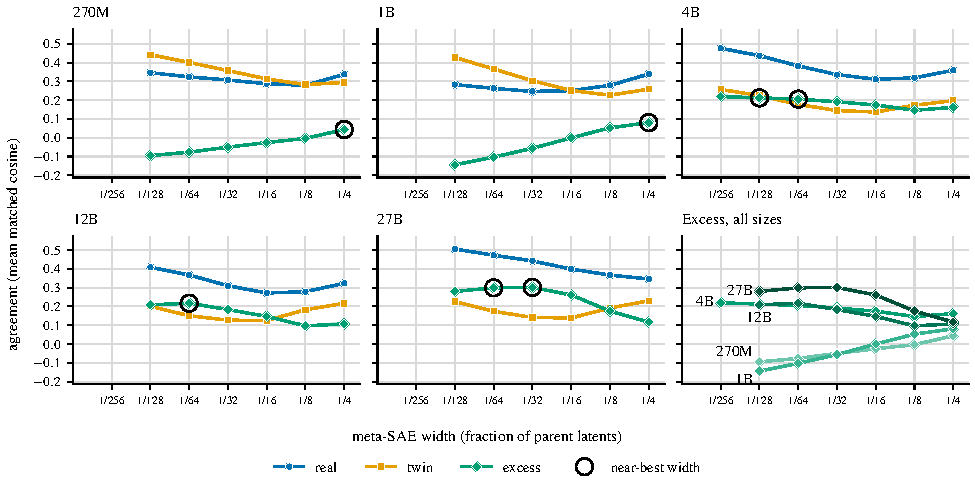
\includegraphics[width=\linewidth]{figures/width.pdf}
  \caption{Real, twin, and excess agreement of the main sweep's meta-SAEs over width at 2,000 epochs. One panel per model size, plus a sixth with all five excess curves. Near-best widths among the six main widths are circled (for 4B, considering 1/256 would shift the near-bests to 1/128 and 1/256). Bands (90\% jackknife intervals over seeds) are all narrower than the markers.}
  \label{fig:width}
\end{figure}

\subsection{Width}

Noise twin raw agreement traces a shallow U over width at every model size (Figure~\ref{fig:width}), bottoming at 1/8 width for Gemma 3 270M and 1B and at 1/16 for sizes 4B and larger.
Real raw agreement is also a shallow U at every size but 27B, where it rises with all narrower widths, and at 1B bottoms out at 1/32 instead of the noise twin's 1/8.

Among the six main widths, 1/128 yields the highest raw real agreement at every size except 1B (where 1/4 is best), but excess agreement reveals a starkly different trend.
Regardless of keeping or dropping dead meta-latents, excess agreement peaks at 1/4 for 270M and 1B and at 1/128, 1/64, and 1/32 for 4B, 12B, and 27B.
Considering excess agreement instead changes the top width for 270M, 27B, and, narrowly, 12B.
Notably, 270M's top width by real raw agreement (1/128) is the worst width by excess agreement ($-$0.095 [$-$0.098, $-$0.093]).

Mean excess interval is negative from 1/8 and smaller for 270M, and from 1/32 and smaller (1/16 after 4k epochs) for 1B.
All widths of both scale sizes show real meta-latents having a greater recurring fraction than their noise counterparts (by 1.4 to 7.2 percentage points, such as 2.5\% vs 0.7\% for 270M's 1/128).

Every size's upturns in raw agreement at 1/4 for both real (except at 27B) and noise twin coincide with a large gap in the real meta-SAEs' explained variance between training and test rows (4.1 to 5.9 times; Appendix~D).
Correspondingly, the split in excess agreement trends between 1B and 4B comes with a jump in dead noise twin meta-latents at 1/4, from 0\% to between 17.1\% and 22.3\%.

\subsection{Model size}

The highest excess agreement seems to increase with model size, from 0.043 at 270M to 0.301 at 27B, though the 4B and 12B tops overlap (Appendix~E) while 270M and 1B's top width is 1/4 but every width from 1/32 to 1/128 at 4B and larger beats 1/4 (top width scores 0.050 to 0.184 more, with intervals above 0).
Live-only excess agreement shows the same ordering.
The jump from 1B to 4B corresponds with lower noise twin agreement at every width (halves for 1/32, from 0.303 to 0.145).
Widths 1/32 to 1/128 at the larger sizes also have 1.9 to 3.3 times the recurring fraction of 1/4 at the same size.
12B and 27B's excess agreements peak at non-end widths (1/64 and 1/32) while 4B peaks at its narrowest (1/256, beating 1/128 by only 0.007 [$-$0.009, 0.024]).

\begin{figure}[t]
  \centering
  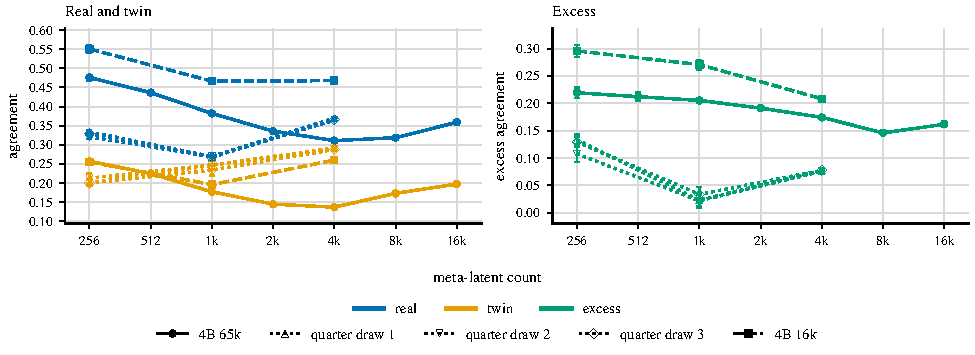
\includegraphics[width=\linewidth]{figures/arms.pdf}
  \caption{At equal steps (26,000), the 4B control meta-SAEs' real, twin, and excess agreement over the number of meta-latents, for meta-SAEs trained on the three quarter draws of the 4B 65k parent's rows and on the 4B 16k parent at widths 1/4, 1/16, and 1/64, and on the 4B 65k parent at 1/4 to 1/256. Error bars are 90\% jackknife intervals over seeds.}
  \label{fig:arms}
\end{figure}

\subsection{What width tracks}

Given equal training steps and the same width or meta-latent count, meta-SAEs trained on the 4B 16k parent score 0.034 to 0.096 higher than those trained on the 4B 65k parent, which themselves score 0.072 to 0.184 higher than those trained on a random quarter of the 4B 65k rows (Figure~\ref{fig:arms}).
It seems that training on fewer rows of the same parent coincides with lower excess agreement at a fixed width or meta-latent count, and that training on a smaller parent can actually raise excess agreement at a fixed count (Appendix~E).
It is also reasonable to say that none of width, meta-latent count, or training row count alone determines excess agreement.

The fifth control, the 270M 16k parent, tests whether a parent's number of latents per hidden dimension explains excess agreement.
It has the same latent count per hidden dimension (25.6) as the 4B 65k parent and a quarter of the 270M 65k parent's 102.4 (Table~\ref{tab:parents}).
Since it also has a quarter of the 270M 65k parent's rows, which by itself lowers excess agreement, only clearly positive excess agreement at narrow widths would support latents per hidden dimension as an explanation.
Given equal training steps, its meta-SAEs show no such gain.
Their excess agreement is 0.049 at width 1/4 (unchanged live-only), $-$0.026 at 1/16 and $-$0.068 at 1/64, each within 0.009 of the 270M 65k parent's at the same width, and only the 1/4 difference excludes 0 (Tables~\ref{tab:app-arms} and~\ref{tab:app-arm-diff}).
At the same meta-latent count, the differences are larger (+0.013 to +0.075), since each partner is a narrower 270M 65k width, where excess agreement is lower.
Thus, latents per hidden dimension alone does not determine excess agreement.

\subsection{Robustness}

\begin{figure}[t]
  \centering
  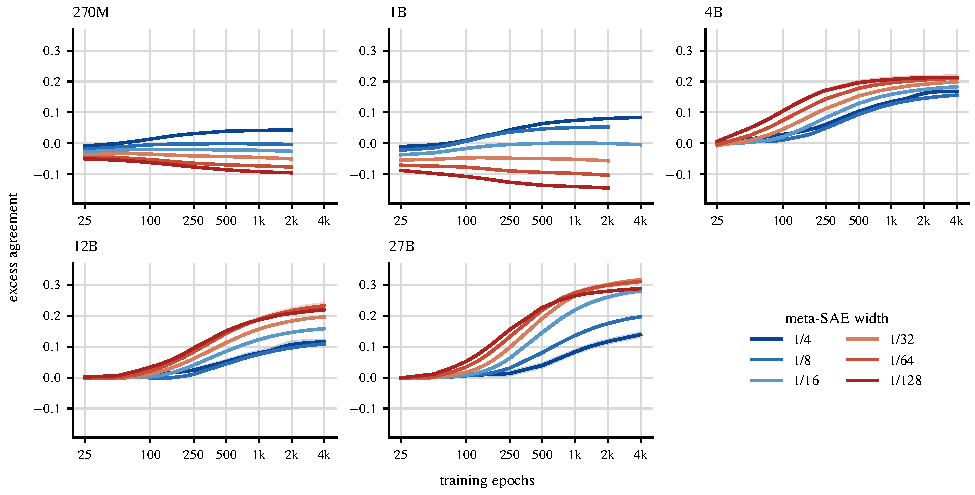
\includegraphics[width=\linewidth]{figures/length.pdf}
  \caption{The six main widths' excess agreement over training epochs (2k or 4k epochs, depending on the training length extension rule), from training snapshots (every 25 epochs up to epoch 250, then every 250 epochs) and the final dictionary, with one panel per model size. Bands are 90\% jackknife intervals over seeds and are mostly narrower than the lines.}
  \label{fig:length}
\end{figure}

\paragraph{Training distance.}
From 4B to 27B, the top and near-best main widths are the same at 2,000 epochs and 4,000 epochs, and the top width's gap above 1/4 moves by at most 0.008.
Even at 4,000 epochs, excess agreement still rising at every 27B width and at 12B widths 1/8 to 1/128 (Figure~\ref{fig:length}) suggests that training had not fully converged.
As for the negative excess for narrow widths on 270M and 1B, overtraining is not to blame since said negative excess appears after just 25 epochs, before 270M's real validation loss bottoms out.
Negative excess agreement on widths 1/64 and 1/128 for 270M also shows in the 1e-3 learning rate check (Appendix~B).
The rate check also shows 27B's narrow widths scoring above 1/4.

\paragraph{Dead latents and the live-only view.}
Dropping dead meta-latents changes no near-best set at any size or length, with or without 1/256.
Dead meta-latents mostly concentrate at width 1/4 for sizes 4B and larger, with the noise twins having more (at 2,000 epochs, 17.1\% to 22.3\% against 1.0\% to 14.5\%), and live-only excess agreement also showing width 1/4 as the worst at both 2,000 and 4,000 epochs.

\section{Discussion}

\paragraph{Choosing a width.}
For Gemma 3 sizes 4B and larger, choose widths 1/32 to 1/128, since they beat 1/4 in excess agreement at both 2,000 and 4,000 epochs, even when using live-only excess agreement (Section~4.2).
Held-out fit (explained variance on test rows) at these sizes varies by at most 0.011 across the six main widths, and at 2,000 epochs, training-row fit falls by 0.285 to 0.329 from 1/4 to 1/128 (Appendix~D).
For 270M and 1B, no main width has more than 2.6\% and 7.7\% of meta-latents recurring, respectively.

\begin{figure}[t]
  \centering
  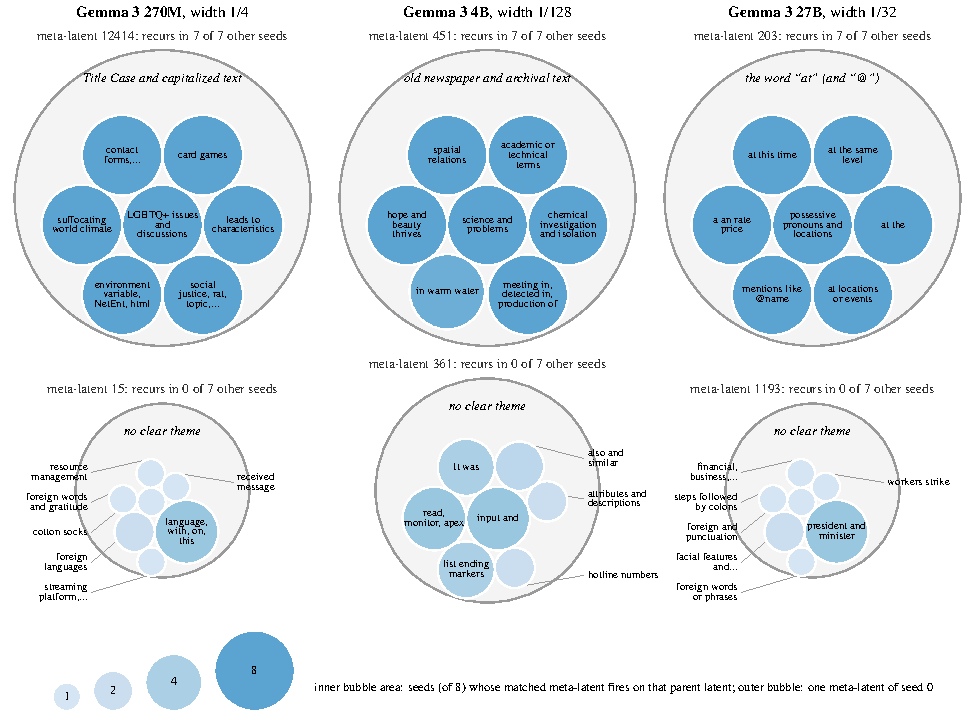
\includegraphics[width=\linewidth]{figures/examples.pdf}
  \caption{Example seed-0 meta-latents that recur in all seven other seeds (top) or in none (bottom), with their seven most strongly activating parent latents and Neuronpedia's automatic labels \citep{lin2023neuronpedia}. Italic descriptions come from three blinded AI readers.}
  \label{fig:examples}
\end{figure}

\paragraph{What the uses rely on.}
Interpretability practitioners commonly analyze individual meta-latents \citep{bussmann2024metasae,leask2025canonical,zhao2026saepp}, and such analyses rely on those meta-latents recurring.
At the main near-best widths for our setups of sizes 4B and larger at 2k epochs, 18.3\% to 27.4\% (19.2\% to 29.9\% at 4k epochs) of meta-latents recur.
At the top main widths for 270M, 4B, and 27B, Figure~\ref{fig:examples} shows the seed-0 meta-latent that recurs in the seven other seeds and also the meta-latent that recurs in none---each chosen as the middle of its group by number of parent latents activated on.
The top parent latents of the recurring meta-latents are activated on in seven to eight of the eight seeds while those for the nonrecurring meta-latents are activated on in at most five, meaning analyses of the nonrecurring meta-latents may not carry over to another seed.
\citet{korznikov2025ortsae} also analyze explained variance of the parent decoder weights, but describe no held-out split.
We found that at \citeauthor{korznikov2025ortsae}'s \citeyearpar{korznikov2025ortsae} width (1/4), our real meta-SAEs explain 4.1 to 5.9 times as much variance on training rows as on test rows (Appendix~D).
We also argue others should prefer excess agreement over raw agreement.

\paragraph{Why.}
Across the five main sweep parents, fewer parent latents per hidden dimension seems to correlate with higher excess agreement, and the 4B 16k parent scores above the 4B 65k parent as this would predict, but the 270M 16k and GPT-2 parents do not fit this trend.
We do not claim to know why the real meta-SAEs agree less than their noise twins at narrow widths for 270M and 1B (Section~4.1) and for the 270M 16k control (Section~4.3), but one hypothesis we offer---with the exception of the GPT-2 parent-based setup---is that the two smallest Gemma 3 models, with their text-only input and small hidden sizes, cannot represent enough broad concepts for a narrow meta-SAE to group the parent's latents as consistently across seeds as a noise twin does by settling along its covariance.
In every main setup, real meta-SAEs fit the test rows better than their noise twins do, but we did not measure how much of that gap comes from the shift in the twins' statistics (Section~3).

\paragraph{Prior findings.}
Our findings of narrower widths of meta-SAEs winning for Gemma 3 4B and larger are similar to how \citet{paulo2025sae} observed SAEs with fewer latents having more seed-to-seed agreement.
Note that their 30\% counts a latent only when both its encoder and decoder match at cosine 0.7, whereas our 29.9\% only counts decoder matches on meta-SAEs.
Also, unlike \citeauthor{liu2026timescale}'s \citeyearpar{liu2026timescale} finding that longer training makes SAE widths more alike in mean max cosine similarity (MMCS, relative to an analytic random-dictionary reference), the top meta-SAE width's lead over 1/4 in excess agreement grows at 12B and 27B from 500 to 4k epochs, shrinking only at 4B (Figure~\ref{fig:length}).

\section{Limitations}

\begin{itemize}
  \item \textbf{One release.}
    Since all of the parent SAEs in the main sweep are Gemma Scope 2 SAEs on Gemma 3, our findings may reflect quirks of this one release rather than general effects.
  \item \textbf{Size moves with other variables.}
    Size also changes alongside hidden size (640 to 5,376), latents per hidden dimension, pretraining tokens (more at 270M than 1B), and whether the model takes image input (from 4B up; Table~\ref{tab:parents}).
    Our assumption of middle layers (after block $N/2$) having comparable representations across Gemma 3 model sizes may also not sufficiently hold due to our larger models potentially having emergent abilities \citep{wei2022emergent} and thus altering what their middle layers represent.
  \item \textbf{Fixed settings.}
    Our findings are largely downstream of just one set of settings we did not vary when measuring agreement: a 3e-3 learning rate, $k$ = 4, 4,096 batch size, 1/32 AuxK weight, and 80/10/10 splits.
    The excess agreement check at 1e-3 only covers four 27B widths and two 270M widths at 2k epochs, but resulted in a reordering of 27B's narrow widths (Appendix~B).
  \item \textbf{Frozen parents only.}
    We did not investigate jointly training the meta-SAE alongside its parent SAE \citep{levinson2026metasaes,zhao2026saepp}, nor \citeauthor{levinson2026metasaes}'s \citeyearpar{levinson2026metasaes} question of meta-SAE width during said joint training.
  \item \textbf{Intervals cover seeds only.}
    The main sweep's excess agreement intervals only sample from meta-SAEs with different seeds, not different training rows.
    However, the three random quarters of the 4B parent's rows resulted in an excess agreement spread that is under the mean seed half-width (half of each draw's 90\% interval) at widths 1/4 and 1/16, but about twice it at 1/64 (Appendix~E).
  \item \textbf{Matryoshka parents.}
    The Gemma Scope 2 technical paper says its SAEs were Matryoshka-trained \citep{mcdougall2025gemmascope2}, and meta-SAEs explain less of a Matryoshka parent's decoder variance than of a BatchTopK parent's \citep{bussmann2025matryoshka,korznikov2025ortsae}, so our findings may not carry over to non-Matryoshka parents.
  \item \textbf{Parents' seed reproducibility unknown.}
    No parent SAE was retrained or compared across seeds.
  \item \textbf{Reproducibility only.}
    Nothing here measures interpretability.
    Higher automated interpretability scores \citep{paulo2025autointerp} are not guaranteed by higher raw or excess agreement across meta-SAE seeds, and we did not investigate whether recurring meta-latents are more easily explainable than nonrecurring meta-latents.
\end{itemize}

\section{Conclusion}

Under the reference configuration, most meta-latents (64.0\%) recur across seeds, compared to only 0.07\% for the noise twins.
As for the sweep's five Gemma Scope 2 parents, which differ from the reference in several ways, they have at most 29.9\% of meta-latents recurring (27B, width 1/32, 4k epochs), while for Gemma 3 270M and 1B, few meta-latents recur (at most 2.6\% and 7.7\%, respectively) and excess agreement ranks 1/4 (the widest main width) as the best.
However, from 4B to 27B, widths 1/32 to 1/128 beat 1/4 on excess agreement at both 2k and 4k epochs (Section~4.2).
Notably, raw and excess agreement pick different top widths for 270M and 27B, and narrowly for 12B (Section~4.1), so we argue that settings carried over to a new parent should be judged by excess agreement over noise twins rather than raw agreement.
Whether these findings hold for other model families, SAE releases, layers and learning rates remains to be tested (Section~6).


\bibliography{references}
\bibliographystyle{tmlr}

\newpage
\appendix

\section{Recipe validation and the reference configuration}
All intervals in these appendices are 90\% leave-one-seed-out jackknife intervals over seeds.

\paragraph{Recipe validation.}
To ensure our recipe reproduces the release \citep{leask2024metasaerelease}, we trained eight real meta-SAEs (seeds 0 to 7).
Note that \citet{leask2025canonical} do not provide a link to the release, so we match the two by owner, name, and settings.
On both our seeds and their release, explained variance is one minus the mean squared residual over the mean squared deviation of the rows from their column mean, with all rows reconstructed as one batch under BatchTopK selection.
Our seeds' explained variance on the training rows (0.5504 to 0.5511) differs from the release's (0.5514) by at most 0.0010, well within our 0.03 tolerance, while no real or twin meta-latent is dead (never active on a training row under the fitted threshold).
\citet{leask2025canonical} report that their meta-SAE explains 55.47\% of the variance, but do not specify how they compute this.

\paragraph{Settings and their sources.}
Certain released configuration fields (Table~\ref{tab:app-settings}) seem ambiguous about how the release's weights were trained, such as the config's epochs field being 5000 while its repository name ends in 0.001\_2000, or aux\_penalty and max\_grad\_norm, which we reasonably infer to be its AuxK weight and clipping threshold, respectively, based only on their field names.

\begin{table}[!htbp]
  \caption{Settings for the reference configuration by source, where \citeauthor{leask2025canonical}'s Appendix A.2 values are for TopK SAEs in general. A blank means that the setting is not in their text, and $\ast$ means it is unknown whether it differs from our unit rows (row norms not recorded).}
  \label{tab:app-settings}
  \centering
  \small
  \begin{tabular}{@{}llll@{}}
    \toprule
    Setting & This study & Leask et al., text & Released config \\
    \midrule
    Meta-latents & 2,304 & 2,304 & dict\_size 2304 \\
    Active per row & k = 4, batch top-k & 4 on average, BatchTopK & top\_k 4, sae\_type topk \\
    Training rows & all 49,152, unit length & 49,152 samples & input\_unit\_norm false$^\ast$ \\
    Epochs & 2,000 & 2,000 & 5000 \\
    Batch & 4,096 & 4,096 & 16384 \\
    Learning rate & 1e-3 & 1e-4 & 0.001 \\
    Adam betas, eps & 0.9, 0.999, 1e-8 & & 0.9, 0.99, no eps field \\
    Gradient clipping & norm 1 & & max\_grad\_norm 100000 \\
    AuxK weight & 1/32 & usually 1/32 (App. A.2) & aux\_penalty 0.0625 \\
    Auxiliary latents & 512 & usually 512 (App. A.2) & top\_k\_aux 512 \\
    Dead after & 5 passes (245,760 rows) & & n\_batches\_to\_dead 100 \\
    \bottomrule
  \end{tabular}
\end{table}

\FloatBarrier\section{Learning-rate tuning}
To help validate our broadly used learning rate of 3e-3, we trained real meta-SAEs with a separate tuning seed (100) at rates 1e-3, 3e-3, and 1e-2 for the main sweep's 30 setups, 4B 65k parent at width 1/256, 4B 16k at three widths, and the 4B 65k's first quarter draw at three widths.
We compared the three rates' validation MSE, measured on the main seeds' held-out rows, at epoch 2k, and looked for gaps larger than 1\%.
Two of the MSE gaps between 3e-3 and the best rate exceeded our 1\% tolerance: the 4B 16k parent (2.01\%) and 12B parent (1.34\%) at width 1/4, where 1e-2 is their best tested learning rate.
Other gaps are at most 0.87\%.
However, we still decided to reuse 3e-3 for these two setups to keep one shared learning rate across all setups.
We did not do learning rate checks for the 270M 16k control parent or the 4B 65k parent's second and third quarter draws at widths 1/4, 1/16, and 1/64, or for the 270M parent at width 1/256.
We also did not do a learning rate check for the noise twins and the reference configuration, since the latter uses its release's 1e-3 learning rate.
Note that the 4B 16k parent and the first quarter draw were compared at 2,000 epochs rather than the 6,500 epochs of their main runs.

\paragraph{Rate check at 1e-3.}
Separate from the learning rate tuning, we also retrained all eight real and noise twin seeds at 1e-3 for 270M (at widths 1/64 and 1/128) and 27B (at widths 1/4, 1/32, 1/64, and 1/128) to see if the width trends were only a result of the shared 3e-3 learning rate.
At \mbox{1e-3}, 270M excess agreement stays negative at widths 1/64 ($-$0.077) and 1/128 ($-$0.080) while 27B excess agreement drops at the four tested widths---by 0.020 [0.006, 0.034] at 1/4, and by 0.073 to 0.033 from 1/32 to 1/128.
However, these drops still keep 27B's narrow widths above 1/4 with non-overlapping intervals, though 1/32 goes from first among them at 3e-3 to last at 1e-3.

\section{Length rule}
When the length rule extends a setup, it continues the same runs, including the twins and the tuning run.
The rule has two tests.
The loss test fires when the seed-100 tuning run at 3e-3 ends with a validation MSE more than 1\% below its value a tenth of the run earlier (at 2,000 epochs, steps 26,000 and 23,400).
The agreement test fires when the eight real seeds' mean agreement rises by more than 0.005 from the halfway snapshot to the final dictionary, without looking at the twins.
If neither test fires, the setup has converged, while if either fires after an extension, we record the setup as not converged without extending it a second time.
Both comparisons are strict, with no margin.
Only the agreement test ever fired (the largest MSE drop was 0.35\%).

\section{Training-row against held-out fit}
Training-row fit is the variance explained on all of a run's own training rows, while held-out fit is the same but on its test rows, with each scored as one batch under batch top-k selection.
Note that a twin's training rows are its own Gaussian rows, while its test rows are the same as the real run's.
At width 1/4, real meta-SAEs explain 4.1 to 5.9 times as much variance on training rows as on held-out rows.
Real held-out fit, on the other hand, stays within 0.118 to 0.139 from 1/4 to 1/128 at 270M and varies by at most 0.011 at each other size (Table~\ref{tab:app-fit}).
Also, real held-out fit beats the twin's in all 30 setups, by 0.015 to 0.060.

\begin{table}[!htbp]
  \caption{Variance explained (training rows / held-out rows) at 2,000 epochs, along with the percent of dead meta-latents at width 1/4, as seed means without intervals. Below 1/4, only the 27B real runs have any dead meta-latents (at most 0.0488\%).}
  \label{tab:app-fit}
  \centering
  \small
  \begin{tabular}{@{}ll*{7}{@{\hspace{6pt}}r}@{}}
    \toprule
    Size & Role & 1/4 & 1/8 & 1/16 & 1/32 & 1/64 & 1/128 & Dead (\%) \\
    \midrule
    270M & real & 0.548/0.134 & 0.400/0.139 & 0.315/0.139 & 0.259/0.137 & 0.221/0.130 & 0.192/0.118 & 0 \\
    & twin & 0.527/0.102 & 0.379/0.109 & 0.288/0.108 & 0.231/0.101 & 0.193/0.090 & 0.165/0.077 & 0 \\
    1B & real & 0.481/0.082 & 0.326/0.082 & 0.233/0.080 & 0.177/0.079 & 0.141/0.078 & 0.117/0.074 & 0.0008 \\
    & twin & 0.454/0.053 & 0.302/0.056 & 0.213/0.057 & 0.160/0.055 & 0.127/0.051 & 0.105/0.046 & 0 \\
    4B & real & 0.454/0.092 & 0.306/0.103 & 0.223/0.103 & 0.175/0.101 & 0.145/0.100 & 0.125/0.097 & 1.0 \\
    & twin & 0.348/0.065 & 0.264/0.070 & 0.183/0.071 & 0.137/0.072 & 0.112/0.073 & 0.097/0.075 & 22.3 \\
    12B & real & 0.420/0.075 & 0.273/0.086 & 0.193/0.086 & 0.150/0.086 & 0.125/0.085 & 0.109/0.083 & 1.7 \\
    & twin & 0.340/0.055 & 0.244/0.060 & 0.166/0.061 & 0.123/0.063 & 0.098/0.065 & 0.085/0.068 & 18.1 \\
    27B & real & 0.393/0.089 & 0.285/0.089 & 0.204/0.090 & 0.157/0.088 & 0.127/0.085 & 0.108/0.082 & 14.5 \\
    & twin & 0.334/0.030 & 0.233/0.044 & 0.157/0.050 & 0.116/0.052 & 0.093/0.054 & 0.080/0.058 & 17.1 \\
    \bottomrule
  \end{tabular}
\end{table}

\section{Full tables}

\subsection{Model size}
Table~\ref{tab:app-size} includes the reference configuration, width 1/4, and every width that is near-best under some view (Section~4.2), each at both 2,000 epochs and its longest training length.
Each of the two views has its own top width and near-best set: the main measure (one-to-one excess agreement over all meta-latents) and live-only (the same but over only live meta-latents).
For the main measure only, we also recorded the top width's lead over 1/4, which is 0.050 [0.039, 0.062], 0.110 [0.094, 0.126] and 0.184 [0.174, 0.194] at 4B, 12B and 27B at 2,000 epochs, compared to 0.046 [0.034, 0.058], 0.118 [0.102, 0.133] and 0.177 [0.166, 0.188] at their longest length, while it is 0 at 270M and 1B since 1/4 is the top width there.
Differences between sizes have no intervals.
With width 1/256 added, 4B's main and live-only near-best sets become \{1/128, 1/256\} at 2,000 epochs, with 1/64 left out by a gap of 0.014 [0.003, 0.025], and \{1/64, 1/128, 1/256\} at 4,000 epochs.
The recurring fraction has no near-best sets or gap intervals; Table~\ref{tab:app-recurring} gives it at every width, without intervals.

\begin{table}[!htbp]
  \caption{Real and twin agreement across model sizes, along with the two views with intervals, at width 1/4 and every width that is near-best under some view, with the reference configuration in the first row. Bold marks each view's top among the six main widths, $\ast$ marks near-best widths that are not the top, and $\dagger$ marks 4B's top with 1/256 included. 270M's 2,000-epoch and longest-length rows coincide.}
  \label{tab:app-size}
  \centering
  \small
  \begin{tabular}{@{}lll*{2}{@{\hspace{5pt}}r}*{2}{@{\hspace{5pt}}l}@{}}
    \toprule
    Parent & Epochs & Width & Real & Twin & Main & Live-only \\
    \midrule
    GPT-2 & 2,000 & 3/64 & 0.737 & 0.338 & 0.400 [0.397, 0.402] & 0.400 [0.397, 0.402] \\
    \midrule
    270M & 2,000 & 1/4 & 0.338 & 0.294 & \textbf{0.043 [0.043, 0.044]} & \textbf{0.043 [0.043, 0.044]} \\
    1B & 2,000 & 1/4 & 0.339 & 0.259 & \textbf{0.080 [0.079, 0.081]} & \textbf{0.080 [0.079, 0.081]} \\
    & 4,000 & 1/4 & 0.342 & 0.258 & \textbf{0.084 [0.083, 0.085]} & \textbf{0.084 [0.083, 0.085]} \\
    4B & 2,000 & 1/4 & 0.359 & 0.197 & 0.162 [0.156, 0.167] & 0.130 [0.128, 0.132] \\
    & & 1/64 & 0.382 & 0.177 & 0.205 [0.202, 0.208]$^\ast$ & 0.205 [0.202, 0.208]$^\ast$ \\
    & & 1/128 & 0.436 & 0.224 & \textbf{0.212 [0.204, 0.220]} & \textbf{0.212 [0.204, 0.220]} \\
    & & 1/256 & 0.476 & 0.257 & 0.219 [0.209, 0.229]$^\dagger$ & 0.219 [0.209, 0.229]$^\dagger$ \\
    & 4,000 & 1/4 & 0.371 & 0.204 & 0.167 [0.161, 0.173] & 0.138 [0.135, 0.140] \\
    & & 1/64 & 0.391 & 0.181 & 0.210 [0.207, 0.214]$^\ast$ & 0.210 [0.207, 0.214]$^\ast$ \\
    & & 1/128 & 0.444 & 0.231 & \textbf{0.213 [0.205, 0.221]} & \textbf{0.213 [0.205, 0.221]} \\
    & & 1/256 & 0.479 & 0.261 & 0.219 [0.209, 0.229]$^\dagger$ & 0.219 [0.209, 0.229]$^\dagger$ \\
    12B & 2,000 & 1/4 & 0.323 & 0.216 & 0.107 [0.095, 0.118] & 0.080 [0.076, 0.083] \\
    & & 1/64 & 0.367 & 0.150 & \textbf{0.217 [0.207, 0.226]} & \textbf{0.217 [0.207, 0.226]} \\
    & 4,000 & 1/4 & 0.340 & 0.226 & 0.115 [0.107, 0.122] & 0.087 [0.082, 0.092] \\
    & & 1/64 & 0.387 & 0.155 & \textbf{0.232 [0.221, 0.243]} & \textbf{0.232 [0.221, 0.243]} \\
    27B & 2,000 & 1/4 & 0.346 & 0.229 & 0.117 [0.108, 0.125] & 0.134 [0.130, 0.138] \\
    & & 1/32 & 0.442 & 0.141 & \textbf{0.301 [0.296, 0.305]} & \textbf{0.301 [0.296, 0.306]} \\
    & & 1/64 & 0.472 & 0.174 & 0.299 [0.292, 0.305]$^\ast$ & 0.299 [0.293, 0.305]$^\ast$ \\
    & 4,000 & 1/4 & 0.379 & 0.239 & 0.139 [0.130, 0.149] & 0.151 [0.146, 0.155] \\
    & & 1/32 & 0.462 & 0.145 & \textbf{0.317 [0.311, 0.322]} & \textbf{0.317 [0.311, 0.322]} \\
    & & 1/64 & 0.488 & 0.177 & 0.311 [0.306, 0.316]$^\ast$ & 0.311 [0.306, 0.316]$^\ast$ \\
    \bottomrule
  \end{tabular}
\end{table}

\begin{table}[!htbp]
  \caption{Model size: recurring fraction (\%) of the real meta-SAEs, with the noise twins' in parentheses, at 2,000 epochs and, for setups the length rule extended, 4,000; means over the 28 seed pairs, no intervals. Blank: not trained at that width or length. Twin fractions under 1\% are coarse (0.0: under 0.05). The reference (GPT-2, width 3/64, 2,000 epochs) has 64.0 (0.07).}
  \label{tab:app-recurring}
  \centering
  \small
  \setlength{\tabcolsep}{4pt}
  \begin{tabular}{@{}llrrrrrrr@{}}
    \toprule
    Parent & Epochs & 1/4 & 1/8 & 1/16 & 1/32 & 1/64 & 1/128 & 1/256 \\
    \midrule
    270M & 2,000 & 2.6 (0.1) & 1.4 (0.0) & 1.7 (0.0) & 1.9 (0.1) & 2.3 (0.2) & 2.5 (0.7) & 4.2 (1.2) \\
    1B & 2,000 & 7.3 (0.1) & 6.4 (0.0) & 4.9 (0.0) & 4.3 (0.0) & 4.6 (0.1) & 4.8 (0.5) & \\
     & 4,000 & 7.7 (0.1) & & 5.3 (0.0) & & & & \\
    4B & 2,000 & 8.6 (0.1) & 11.1 (0.0) & 14.0 (0.1) & 16.2 (0.2) & 18.3 (0.4) & 20.0 (0.9) & 20.2 (2.0) \\
     & 4,000 & 9.6 (0.1) & 12.0 (0.0) & 14.8 (0.1) & 17.1 (0.2) & 19.2 (0.4) & 20.6 (0.8) & 20.7 (2.0) \\
    12B & 2,000 & 6.1 (0.4) & 8.6 (0.1) & 12.8 (0.1) & 17.2 (0.2) & 20.5 (0.3) & 19.4 (0.8) & \\
     & 4,000 & 7.1 (0.4) & 9.6 (0.1) & 14.3 (0.1) & 19.2 (0.2) & 22.8 (0.3) & 21.0 (0.8) & \\
    27B & 2,000 & 12.1 (0.6) & 17.8 (0.1) & 24.3 (0.1) & 27.4 (0.3) & 27.1 (0.6) & 27.8 (1.1) & \\
     & 4,000 & 14.5 (0.7) & 20.7 (0.1) & 27.2 (0.1) & 29.9 (0.3) & 29.3 (0.6) & 29.3 (1.1) & \\
    \bottomrule
  \end{tabular}
\end{table}

\subsection{Controls}
Each quarter draw's twin trains on its own quarter of the 4B 65k parent's noise rows.
At width 1/4 and 2,000 epochs, 33.9\% of the 4B 16k parent's real meta-latents are dead, compared to 1.5\% for its twins, while neither has any dead meta-latents at 6,500 epochs.

\begin{table}[!ht]
  \caption{Excess agreement of the controls, with intervals. Control widths are fractions of 16,384 rows (4,096, 1,024 and 256 meta-latents), while 65k widths are fractions of 65,536 rows (16,384, 4,096 and 1,024 meta-latents). At width 1/256 (256 meta-latents), 4B 65k scores 0.219 [0.209, 0.229] and 270M 65k scores $-$0.081 [$-$0.091, $-$0.071].}
  \label{tab:app-arms}
  \centering
  \small
  \begin{tabular}{@{}llll@{}}
    \toprule
    Epochs, control & 1/4 & 1/16 & 1/64 \\
    \midrule
    2,000, quarter draw 1 & 0.060 [0.059, 0.062] & 0.025 [0.013, 0.037] & 0.124 [0.115, 0.133] \\
    2,000, quarter draw 2 & 0.060 [0.058, 0.063] & 0.022 [0.013, 0.032] & 0.107 [0.097, 0.117] \\
    2,000, quarter draw 3 & 0.061 [0.057, 0.065] & 0.033 [0.021, 0.046] & 0.121 [0.114, 0.128] \\
    2,000, 4B 16k & 0.052 [0.042, 0.062] & 0.257 [0.252, 0.262] & 0.290 [0.280, 0.301] \\
    2,000, 270M 16k & 0.047 [0.044, 0.049] & $-$0.017 [$-$0.020, $-$0.014] & $-$0.055 [$-$0.063, $-$0.046] \\
    2,000, 4B 65k & 0.162 [0.156, 0.167] & 0.174 [0.172, 0.176] & 0.205 [0.202, 0.208] \\
    2,000, 270M 65k & 0.043 [0.043, 0.044] & $-$0.026 [$-$0.027, $-$0.024] & $-$0.077 [$-$0.081, $-$0.073] \\
    \midrule
    6,500, quarter draw 1 & 0.077 [0.075, 0.079] & 0.023 [0.010, 0.036] & 0.133 [0.123, 0.143] \\
    6,500, quarter draw 2 & 0.076 [0.073, 0.079] & 0.022 [0.012, 0.032] & 0.108 [0.093, 0.122] \\
    6,500, quarter draw 3 & 0.078 [0.074, 0.081] & 0.033 [0.019, 0.048] & 0.129 [0.120, 0.138] \\
    6,500, 4B 16k & 0.208 [0.205, 0.211] & 0.271 [0.262, 0.279] & 0.296 [0.285, 0.306] \\
    6,500, 270M 16k & 0.049 [0.047, 0.051] & $-$0.026 [$-$0.029, $-$0.023] & $-$0.068 [$-$0.076, $-$0.060] \\
    \bottomrule
  \end{tabular}
\end{table}

\begin{table}[!ht]
  \caption{Difference in excess agreement between each control and its matching 65k parent (control minus 65k parent), with intervals. For the same meta-latent count, the control's widths 1/4, 1/16 and 1/64 are compared with the 65k parent's 1/16, 1/64 and 1/256, respectively. For equal steps, the control is at 6,500 epochs and the 65k parent at 2,000.}
  \label{tab:app-arm-diff}
  \centering
  \small
  \begin{tabular}{@{}l*{2}{@{\hspace{6pt}}l}@{}}
    \toprule
    Control, width & Same width, equal steps & Same count, equal steps \\
    \midrule
    Draw 1, 1/4 & $-$0.085 [$-$0.090, $-$0.079] & $-$0.097 [$-$0.100, $-$0.095] \\
    Draw 1, 1/16 & $-$0.151 [$-$0.164, $-$0.139] & $-$0.182 [$-$0.197, $-$0.168] \\
    Draw 1, 1/64 & $-$0.072 [$-$0.082, $-$0.062] & $-$0.086 [$-$0.103, $-$0.069] \\
    Draw 2, 1/4 & $-$0.086 [$-$0.090, $-$0.081] & $-$0.098 [$-$0.101, $-$0.096] \\
    Draw 2, 1/16 & $-$0.152 [$-$0.163, $-$0.142] & $-$0.184 [$-$0.195, $-$0.172] \\
    Draw 2, 1/64 & $-$0.098 [$-$0.112, $-$0.083] & $-$0.112 [$-$0.127, $-$0.096] \\
    Draw 3, 1/4 & $-$0.084 [$-$0.089, $-$0.079] & $-$0.097 [$-$0.100, $-$0.093] \\
    Draw 3, 1/16 & $-$0.141 [$-$0.156, $-$0.126] & $-$0.172 [$-$0.186, $-$0.158] \\
    Draw 3, 1/64 & $-$0.076 [$-$0.086, $-$0.066] & $-$0.090 [$-$0.103, $-$0.077] \\
    4B 16k, 1/4 & 0.047 [0.040, 0.053] & 0.034 [0.031, 0.037] \\
    4B 16k, 1/16 & 0.096 [0.088, 0.105] & 0.065 [0.056, 0.075] \\
    4B 16k, 1/64 & 0.090 [0.078, 0.103] & 0.077 [0.061, 0.092] \\
    270M 16k, 1/4 & 0.006 [0.003, 0.008] & 0.075 [0.072, 0.078] \\
    270M 16k, 1/16 & $-$0.000 [$-$0.003, 0.003] & 0.051 [0.046, 0.056] \\
    270M 16k, 1/64 & 0.009 [$-$0.001, 0.018] & 0.013 [0.000, 0.025] \\
    \bottomrule
  \end{tabular}
\end{table}

\subsection{Quarter-draw spread}
With only three draws, we get a range rather than a standard error, so this comparison is descriptive only.
At 2,000 epochs, the draws' excess agreement spreads by 0.001, 0.011 and 0.017 at widths 1/4, 1/16 and 1/64 (0.002, 0.012 and 0.025 at 6,500 epochs), compared to their own 90\% half-widths of 0.001 to 0.004, 0.009 to 0.012 and 0.007 to 0.010 (0.002 to 0.003, 0.010 to 0.014 and 0.009 to 0.015 at 6,500 epochs).
Only at 1/64 does the spread exceed every draw's half-width, at 1.6 to 2.4 times the half-width (1.7 to 2.8 times at 6,500 epochs).
This is our only evidence on variation across row samples, and only at 13,107 training rows.

